%#!platex --src-specials main.tex

\chapter{触覚の生理学的特徴と\\関連する先行研究}
\label{chap:haptic}
本章において,  触覚の生理学的特徴, 触覚情報の取り扱いに関する先行研究について概説する.  

\section{触覚の生理学的特徴}
\subsection{ヒトの皮膚構造}
ヒトの触覚は成人にして約\,1.6$-$1.8\,$\mathrm{m^2}$の面積と\,3$-$5\,$\mathrm{kg}$の重量を持つ最大の感覚器官であり,  身体で最も大きな器官で全体重のほぼ1/6の重さを占める.  皮膚は表皮, 真皮, 皮下組織の三層構造からなり, この皮膚内部に時空間的に異なる特性を持つ触覚受容器が固有の位置に分布している. 皮膚構造を以下の図\ref{fig:skin}に示す. 
\begin{figure}[H]
\begin{center}
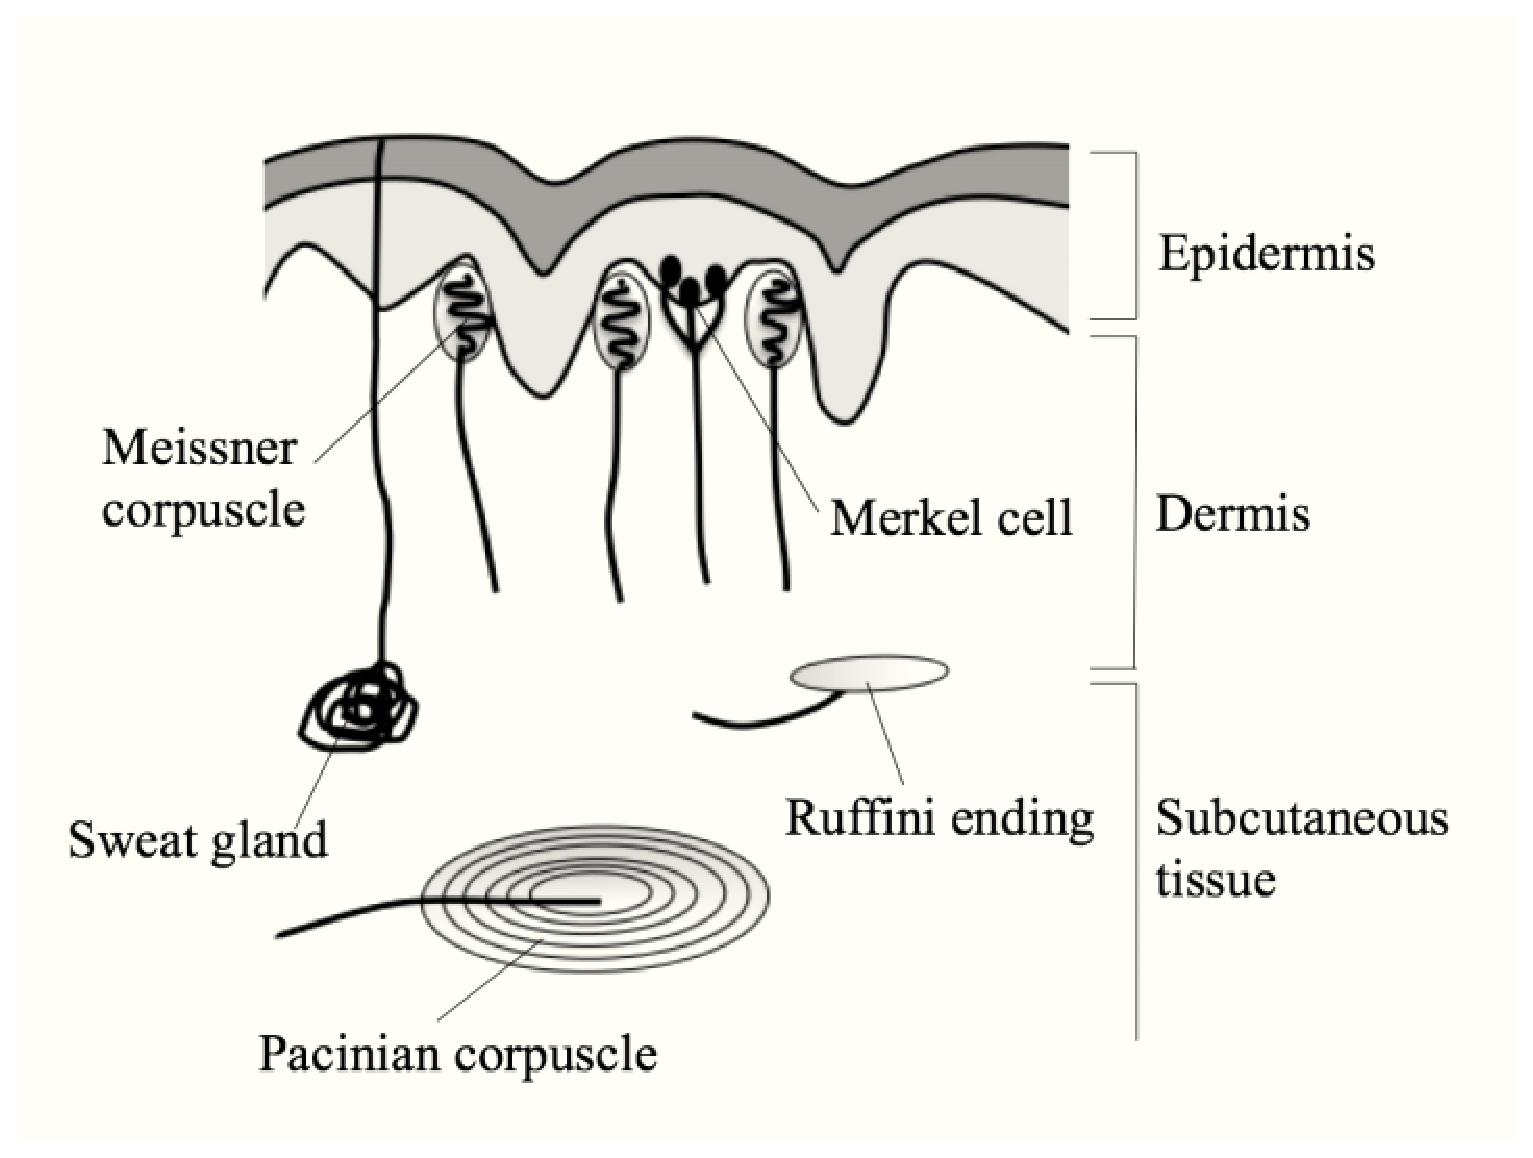
\includegraphics[width=8cm]{eps/skin_str.eps}
\caption{皮膚構造(\cite{mechanizm}より引用)}
\label{fig:skin}
\end{center}
\end{figure}

\subsection{触覚受容器}
無毛部皮膚に存在する触覚受容器において,  表皮の最深部に存在するメルケル小体 (Merkel discs), 真皮の最外層にあるマイスナー小体 (Meissner corpusde), 深層にあるパチニ小体 (Pacini corpuscle), ルフィニ終末 (Ruffini ending) の 4 つがよく知られている.
4つの受容器は応答の速さの違いから,  それぞれ\,Fast Adapting : FA,  \,Slow Adapting : SA に分類される \cite{1984438}.
また,  そこから触覚受容器の応答できる皮膚表面の範囲,  受容野の広さの違いからタイプ\rm\,I\,,  タイプ\rm\,II\,に分類される. 
これらの受容特性を表\ref{tab:Receptors}に示す \cite{前野隆司2000器用な手}.%\cite{2000772}.

\begin{table}[H]
 \caption{tactile receptors at glabrous skin}
 \label{tab:Receptors}
 \begin{center}
 \scalebox{0.8}{
\begin{tabular}{cllll}
\hline
Receptors          & type                                                     & receptive field & adaptation rate & size                                                              \\ \hline
Meissner corpuscle & FA\rm\,I\,  & small           & fast            & $L = 20-150\, \mathrm{\mu m},\, D = 40-70\, \mathrm{\mu m}$ \\
Merkel discs       & SA\rm\,I\,  & small           & slow            & $D = 7\, \mathrm{\mu m},\,T = 1\, \mathrm{\mu m}$           \\
Pacinian corpuscle & FA\rm\,II\, & large           & very fast       & $L = 0.3-1.5\, \mathrm{mm},\, D = 0.2-0.7\, \mathrm{mm}$    \\
Ruffini ending     & SA\rm\,II\, & large           & slow            & $L = 0.5-2\, \mathrm{mm},\, D = 0.2\, \mathrm{mm}$          \\ \hline
                   &                                                          &                 &                 & ($L : length, D : diameter, T : tickness$)                       
\end{tabular}
}
\end{center}
\end{table}

また,  皮膚表面に振動刺激を与えた際の FA\rm\,I\,(メルケル小体),  SA\rm\,I\,(マイスナー小体),   FA\rm\,II\,(パチニ小体) の振動検出閾値と振動刺激周波数との関係を以下の図\ref{fig:rece}に示す \cite{前野隆司2000器用な手}.%\cite{2000772}\cite{inproceedings}. 
 図\ref{fig:rece}より,  SA\rm\,I\,の振動検出閾値は極小値が\,3$-$5\,$ \mathrm{Hz}$であるが,  刺激の周波数にほぼ影響されることなく検出を行う.  FA\rm\,I\,は数\,10\,$ \mathrm{Hz}$, FA\rm\,II\,は\,200$-$300\,$ \mathrm{Hz}$付近で極小値を得て高い感度を発揮する. これらから触覚は様々な周波数帯域の信号を受容をできるようなっており, 各受容器の棲み分けがなされているといえる. 
前述の通り各受容器の存在する深度も違い, 皮膚を通して伝わる信号は空間周波数フィルタを通された信号のようになることから, 伝達する信号の鮮明度も各受容器ごとに変わってくる. 以上より各受容器は時間周波数, 空間周波数をそれぞれ分担して検出している. 
\begin{figure}[H]
    \begin{center}
    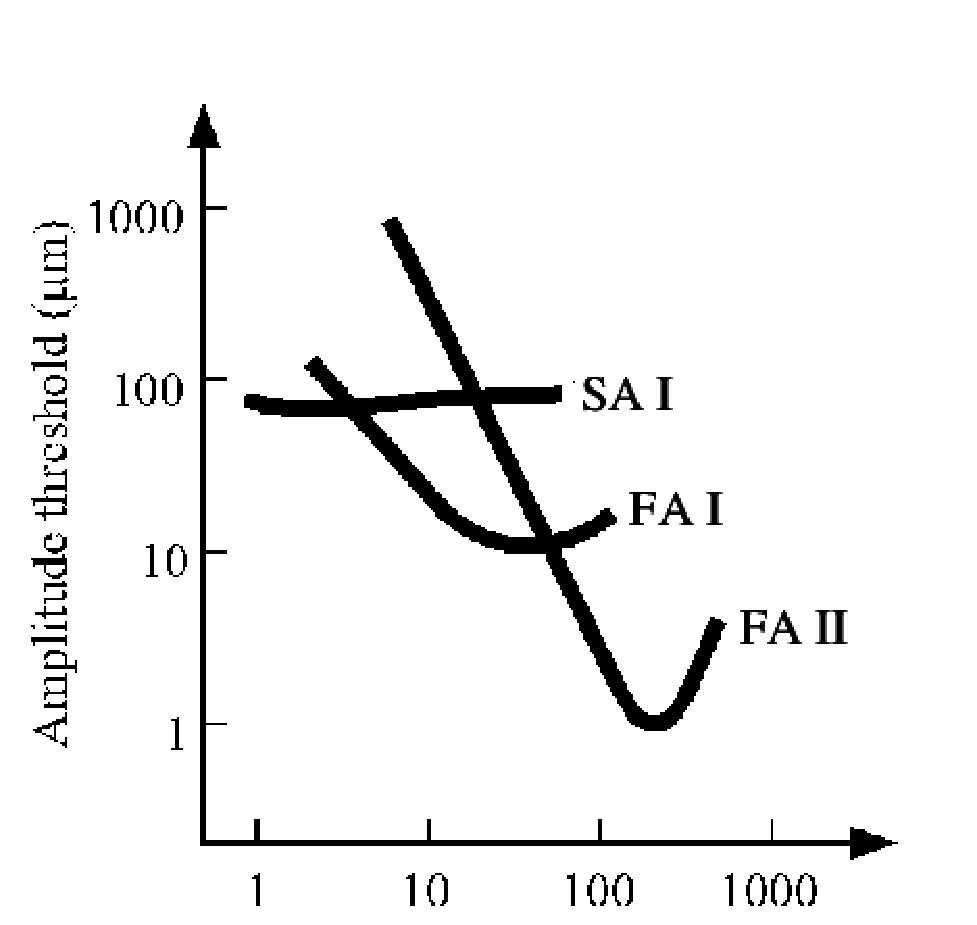
\includegraphics[width=8cm]{eps/threshold.eps}
    \caption{受容器の振動検出(\cite{maeno}より)}
    \label{fig:rece}
   \end{center}
   \end{figure}
   
\section{触覚情報の取扱に関する研究}
触覚ディスプレイを用いた情報提示の前段階として, テクスチャの触覚データを加速度情報として取得する研究が広く行われている.  Abdulali らは収集した加速度触覚情報をニューラルネットワークの1種である Radial Basis Function Network を用い分類を行った\cite{abdulalis}.   Strese らはユークリッド距離, マハラノビス距離, GMM の3種の機械学習アルゴリズムをそれぞれを使用し分類を行い, 精度比較を行っている\cite{strese2016multimodal}. また, Jamali らは単純ベイズ分類器を用いて分類を行った \cite{jamali2010material}. 
また, 機械学習で分類を行うにあたって, 入力に次元削減を施している研究も見受けられる. 
 Mengqi らはオートエンコーダと畳み込みニューラルネットワークを組み合わせた ACNN というネットワークを用い分類を行っている\cite{mengqi}. この際用いられている手法が J. Kuchenbecker らによって提案された DFT321 \cite{dft321} と呼ばれる次元削減アルゴリズムである. この手法は同様に畳み込みニューラルネットワークで触覚情報の分類を行った Zheng ら \cite{zheng2016deep} やTawfique ら \cite{Tawfique} も入力の前処理として使用している. しかし, 同じ3軸加速度データを扱う研究でも人の行動分析の場合, 3軸加速度をそのまま入力とする研究も多く見られる \cite{active_recog}. 
 
 これらの先行研究に対し, 本研究ではテクスチャの分類問題に対して, 次元削減の妥当性の検証として基本的かつシンプルな畳み込みニューラルネットワークを構築し, 次元削減を行った場合の3軸加速度触覚情報と次元削減を行わない場合の3軸加速度触覚情報で分類精度の観点から性能にどの程度差が生じるか比較を行う. また, 畳み込みニューラルネットワークで一般に用いられる特徴量ごとの正規化を3軸加速度触覚情報にも適用し, 正規化を行わない場合の分類精度との比較を行う.

% Local Variables:
% TeX-master: "main"
% mode: yatex
% End:
